
\subsection{Mathematical Formulation}

The bondholder has the option to convert the bond into shares only at specific discrete times:
\begin{itemize}
    \item After each coupon payment date $t_i$,
    \item At final maturity $T$.
\end{itemize}

I assume the stock price $S(t)$ follows a stochastic process under the risk-neutral measure. Define $V(t, S)$ as the value of the convertible bond at time $t$ when the stock price is $S$.

The dynamic programming (backward induction) recursion is formulated as follows:
\begin{itemize}
    \item \textbf{At maturity} $T$:
    \begin{equation}
        V(T, S) = \max\left( N, \ell S \right),
    \end{equation}
    reflecting the choice between receiving the bond's face value or converting into shares at maturity.
    
    \item \textbf{At coupon payment dates} $t_i$:
    \begin{equation}
        V(t_i, S) = \max \left\{
            e^{-r \Delta t} \mathbb{E} \left[ V(t_{i+1}, S') \mid S(t_i) = S \right] + c N \Delta t, \;
            \ell S
        \right\},
    \end{equation}
    where:
    \begin{itemize}
        \item $\mathbb{E}[\cdot]$ denotes the risk-neutral expectation,
        \item $K N \Delta t$ is the coupon payment received at $t_i$.
    \end{itemize}
    
    \item \textbf{At non-coupon payment dates} (no conversion allowed):
    \begin{equation}
        V(t, S) = e^{-r \Delta t} \mathbb{E} \left[ V(t + \Delta t, S') \mid S(t) = S \right].
    \end{equation}
\end{itemize}

At each coupon date and at maturity, the bondholder optimally chooses between:
\begin{itemize}
    \item Continuing to hold the bond (receiving future coupon payments and principal at maturity),
    \item Early conversion into shares.
\end{itemize}

\vspace{0.3cm}
\noindent
The expectation $\mathbb{E}[\cdot]$ is evaluated using a binomial tree discretization of the stock price dynamics under the risk-neutral measure and Monte-Carlo methods.

\subsection{Binomial Trees Method}

To solve the dynamic programming recursion, the time interval $[0, T]$ is discretized into $N_{\text{steps}}$ steps of size $\Delta t = T / N_{\text{steps}}$. A finer grid is used with monthly steps, while conversion opportunities are restricted to semiannual coupon dates. A binomial tree is constructed to model the evolution of the stock price $S(t)$. \\ At each time step:
\begin{itemize}
    \item The stock price can move up by a factor $u = e^{\sigma \sqrt{\Delta t}}$ or down by a factor $d = 1/u$.
    \item The risk-neutral probability $p$ of an upward move is given by:
    \begin{equation}
        p = \frac{e^{r \Delta t} - d}{u - d}.
    \end{equation}
\end{itemize}

At each node:
\begin{itemize}
    \item The \textbf{continuation value} is computed as the discounted expected value of future bond values plus coupon payments (if at a coupon date):
    \begin{equation}
        \text{Continuation Value} = e^{-r \Delta t} \left( p V_{\text{up}} + (1 - p) V_{\text{down}} \right) + K N \Delta t.
    \end{equation}
    \item The \textbf{conversion value} is:
    \begin{equation}
        \text{Conversion Value} = \ell S.
    \end{equation}
\end{itemize}

At coupon dates:
\begin{equation}
    V(t_i, S) = \max \left( \text{Continuation Value}, \text{Conversion Value} \right),
\end{equation}
and at non-coupon dates, only continuation is allowed:
\begin{equation}
    V(t, S) = \text{Continuation Value}.
\end{equation}

At maturity:
\begin{equation}
    V(T, S) = \max(N, \ell S).
\end{equation}


The following parameters are used for the numerical simulation:
\begin{itemize}
    \item Initial stock price: $S_0 = 200$
    \item Face value: $N = 1000$
    \item Conversion ratio: $\ell = 3$
    \item Annual coupon rate: $K_{\text{coupon}} = 0.016$
    \item Risk-free rate: $r = 0.03$
    \item Volatility: $\sigma = 0.3$
    \item Maturity: $T = 5$ years
    \item Number of time steps: $N_{\text{steps}} = 60$ (monthly steps)
\end{itemize}

\begin{figure}[h!]
    \centering
    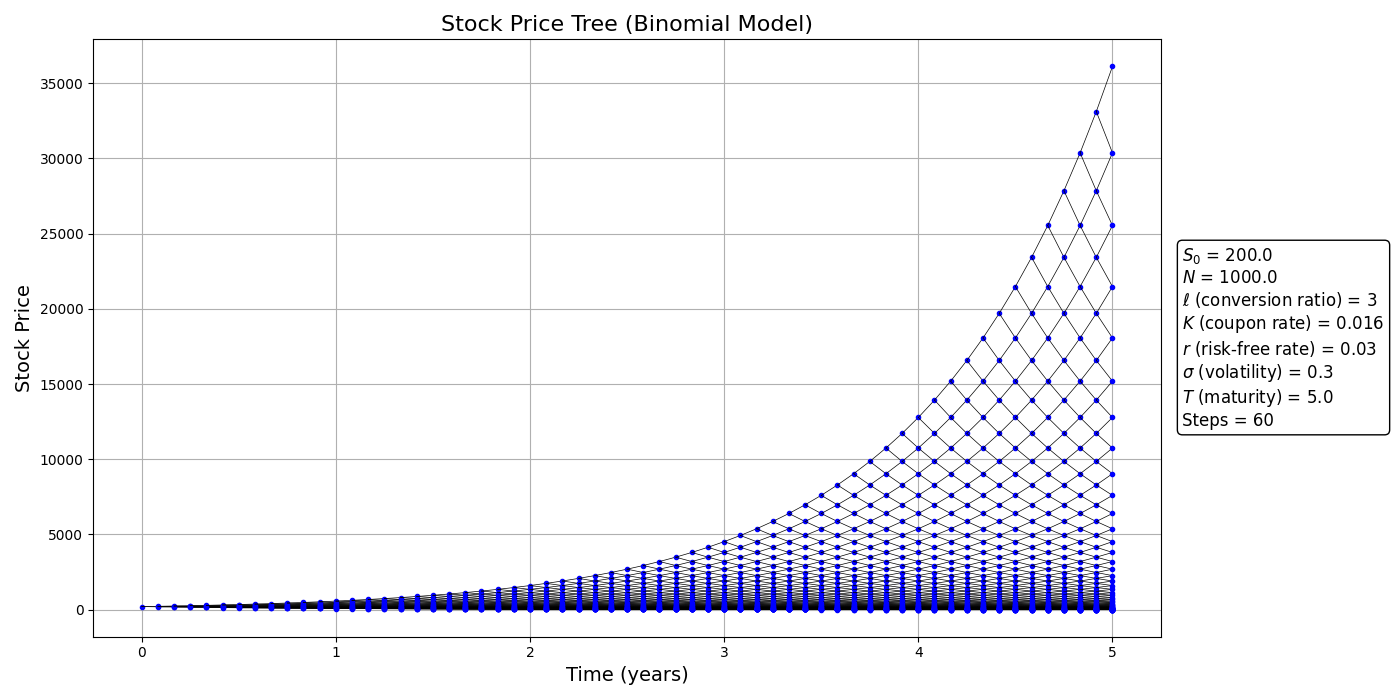
\includegraphics[width=0.65\linewidth]{13_ConvertibleBonds/img/01_StockPrice.png}
    \caption{Stock Price Tree (Binomial Model)}
    \label{fig:01_stock_price}
\end{figure}


\begin{figure}[h!]
    \centering
    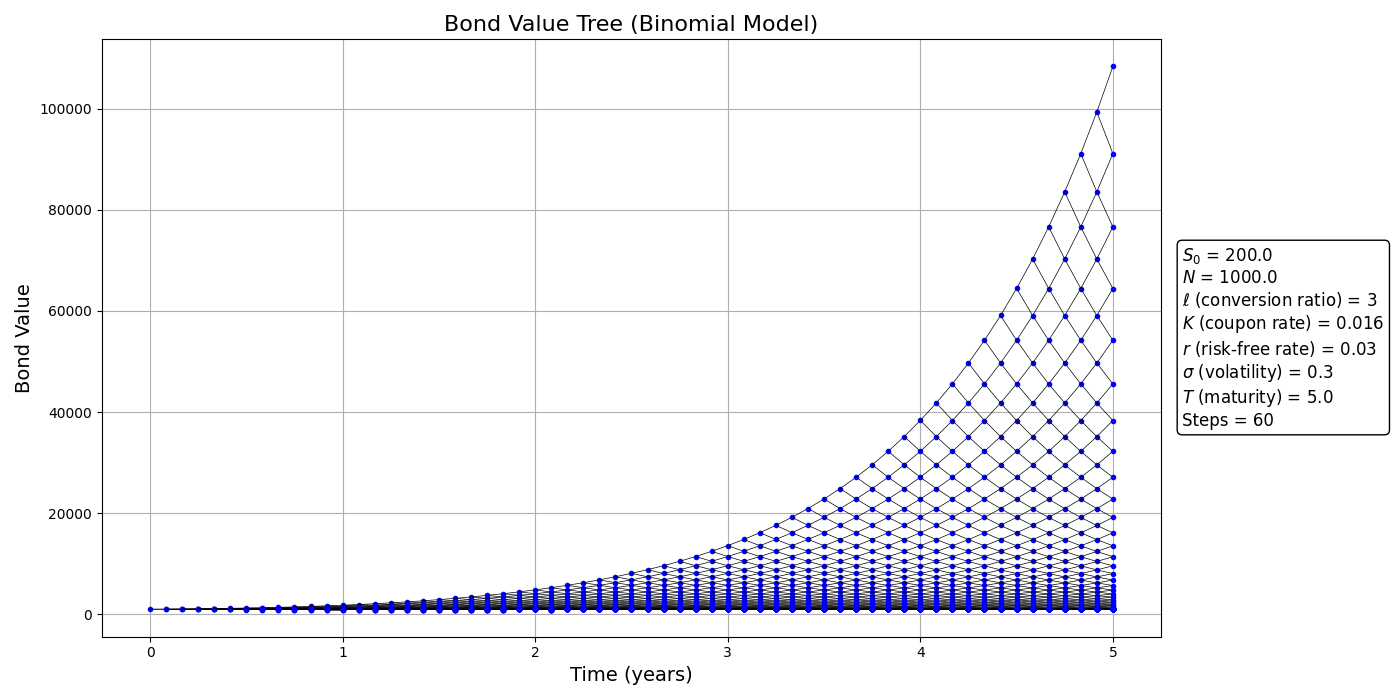
\includegraphics[width=0.65\linewidth]{13_ConvertibleBonds/img/01_BondValue.png}
    \caption{Bond Value Tree (Binomial Model)}
    \label{fig:01_bonds_price}
\end{figure}


Using the binomial tree method with the above parameters, the computed price of the convertible bond at $t = 0$ is:
\begin{equation}
    V(0, S_0) = 1014.16
\end{equation}

